\chapter{Moving least squares}
In this section concept of the Moving Least Squares (MLS) will be described. The MLS approximation was introduced in an early paper by Lancaster and Salkauskas  \cite{MLSSalkauskas} in 1981 with special cases going back to McLain  \cite{MLSMcLain1}, \cite{MLSMcLain2} in 1974 and 1976. Since in MLS one writes the value of the unknown function in terms of scattered data, it can be used as an approximation to span the trial space in meshless (or meshfree) methods. This approximation has found many applications in curve fitting and numerical solutions of partial differential equations.

Most of the theoretical material was taken from \cite{MLSIntro}.
\section{Global least squares}
\textbf{Problem domain.} Given a points $X = [x_1, ..., x_n]$. The goal is to fit a point cloud to some geometric surface e.g. sphere. Suppose, that we are given a values of $u(X) = [u_1, ..., u_n]$ and the values are biased, e.g. $u_i + \varepsilon = u(x_i)$ and the function $u(x)$ is unknown.

The idea of a Global Least Squares (GLS) technique is to reconstruct $u(x)$ so that for all $|u_i - u(x_i)|$ is minimal, that is:
\begin{equation}
	argmin(\sum_i (u_i - u(x_i))^2)
	\label{eq:min_problem}
\end{equation}
\textbf{Description.} For simplicity 1D problem will be reviewed e.g. $x_i \in R$. Function $u(x_i)$ can be described as a polynomial $u(x)=\sum_k{c_i \cdot x^k}$, where $c_i$ are unknown coefficients, which are to be found.
As soon as in the problem domain $x_i$ are given values we can substitute a $x^k$ with a coefficient $b_k(x) = x^k$. Returning to \ref{eq:min_problem} the equation can be expanded the minimization problem:
\begin{equation}
	\sum_i (u_i - \sum_j{c_j \cdot b_j(x_i)})^2 = R^{GLS}
	\label{eq:min_problem_exp}
\end{equation}
where $R^{GLS}$ is a function to be minimized. To find a minimum, the first derivative of the equation \ref{eq:min_problem_exp} w.r.t. $c_j$ should be taken, and assigned to 0. An example of one derivative over $c_k$ is in Equation \ref{eq:RGLSderivatieve}
\begin{equation}
	\dfrac{\partial R^{GLS}}{\partial c_k} = 2\cdot \sum_i{b_k(x_i) \cdot (\sum_j{b_j(x_i)\cdot c_j} - u_i)} = 0
	\label{eq:RGLSderivatieve}
\end{equation}
or equation \ref{eq:RGLSderivatieve}  can be rewritten as follows:
\begin{equation}
	\sum_i{b_k(x_i) \cdot (\sum_j{b_j(x_i)\cdot c_j})}  = \sum_i {b_k(x_i) \cdot u_i}
	\label{eq:RGLSderFinal}
\end{equation}
Taking all partial derivatives over $c_j$ the set of equations can be generated $LS = 
\begin{matrix}
	\sum_i{b_1(x_i) \cdot (\sum_j{b_j(x_i)\cdot c_j})}  &= \sum_i {b_1(x_i) \cdot u_i}\\
	\sum_i{b_2(x_i) \cdot (\sum_j{b_j(x_i)\cdot c_j})}  &= \sum_i {b_2(x_i) \cdot u_i}\\
	\sum_i{b_3(x_i) \cdot (\sum_j{b_j(x_i)\cdot c_j})}  &= \sum_i {b_3(x_i) \cdot u_i}\\
	...\\
	\sum_i{b_m(x_i) \cdot (\sum_j{b_j(x_i)\cdot c_j})}  &= \sum_i {b_m(x_i) \cdot u_i}\\
\end{matrix}$.

This is a linear system with m equations and m unknown $c_j$`s. Thus it can be reformulated into a matrix form
\begin{equation}
 B \cdot B^T \cdot c  = B\cdot u
 \label{eq:matrEquation}
\end{equation}
where $B = 
\begin{pmatrix}
	b_1(x_1) & b_1(x_2) & ... & b_1(x_n)\\
	b_2(x_1) & b_2(x_2) & ... & b_2(x_n)\\
	...\\
	b_m(x_1) & b_m(x_2) & ... & b_m(x_n)\\
\end{pmatrix}$, $u = \
\begin{pmatrix}
	u_1\\
	u_2\\
	...\\
	u_n
\end{pmatrix}$ is a vector of the given scalar function values, and $c = 
\begin{pmatrix}
	c_1\\
	c_2\\
	...\\
	c_m
\end{pmatrix}$ are the unknown coefficients of the searched function. Thus the solution of \textbf{c} can be retrieved by solving a linear system formulated by the matrix equation \ref{eq:matrEquation}.

Having obtained the coefficients \textbf{c}, we can then compute the value of the function at any point $x$ in the domain using the equation for $u(x)$ . This analysis is substantially unchanged in higher dimensions. An example of a global least squares fit is shown in Figure \ref{fig:gls_example}.
\begin{figure}[h]
	\begin{center}
		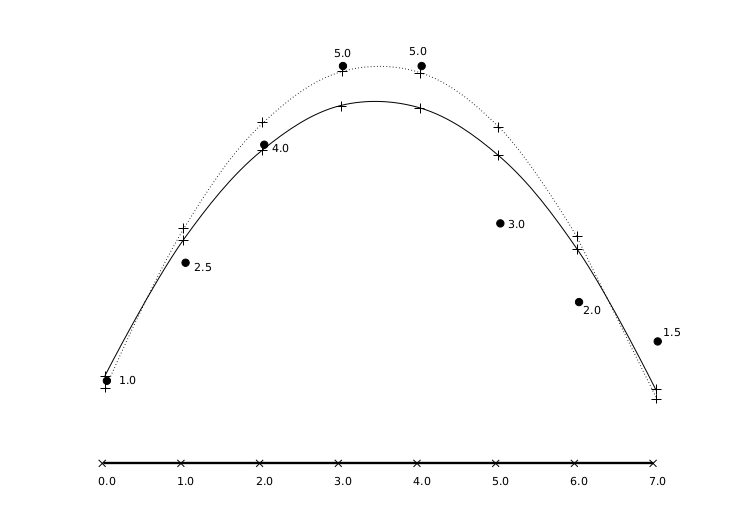
\includegraphics[width=0.7\textwidth]{figures/GLS.png}
	\end{center}
	\caption{Global Least Squares (solid curve) and Weighted Global Least Squares (dashed curve) fit for data represented by the solid circles. The fit is a quadratic fit. The weighting used for the dashed curve is 1.0 every where except at x = 3.0 and x = 4.0 where it is 10.0 (\cite{MLSIntro})}
	\label{fig:gls_example}
\end{figure}
\section{Weighted GLS}
We can assign each data value a weight w to use in the least squares fit, so that we write the objective function to be minimized as:
\begin{equation}
	R^{WGLS} = \sum_i{w_i \cdot (u_i - u(x_i)^2} = \sum_i{w_i \cdot (u_i - \sum_j{b_j(x_i)\cdot c_j})^2}
\end{equation}
The gradient $\nabla_c R^{WGLS}$ is expanded to a linear system:
\begin{equation}
	B^TWBc = B^TWu
\end{equation}
where $W$ is a diagonal matrix of the form:\\
$W = \begin{pmatrix}
	w_1 & 0 	& ... & 0\\
	0 	& w_2 	& ... & 0\\
	...\\
	0 	& 0 	& ... & w_n\\
\end{pmatrix}$\\
with $W_{i,i} = w_i$. Figure \ref{fig:gls_example} shows an example of a weighted global least-squares approximation.

The solution is obtained by solving equation \ref{WGLS_SLAU}
\begin{equation}
	c = (B^TWB)^{-1}\cdot B^TWu \label{WGLS_SLAU}
\end{equation}
\section{Weighted Local Least Squares}
In global least-squares fitting, we assumed that the function represented by the data can be accurately captured by a single polynomial spanning the entire domain. For large, complex data sets, however, this would require to fit a polynomial of an impractically high order, and even then it may not capture all the features of the data. So instead of a global solution, a better picture of the solution can be obtained by fitting lower order polynomials to each data point $(x_p, u_p)$ and its neighbors. Thus there are N least-squares fits $u_i(x)$ , each one approximating the solution at point $x_i$ and the coefficient vector $c_i$ is different at each point.

The approximate solution for point $x_p$ is evaluated through $R^{WLLS}_p = \sum_i^N w_{pi} \cdot (u_i - u(x_i))^2$, where $i\in [1, N]$ are neighbors of $x_p$. The gradient is expanded to matrix equation: $B^T W_p Bc_p = B_p^T W_p u$.

\begin{figure}[H]
	\begin{center}
		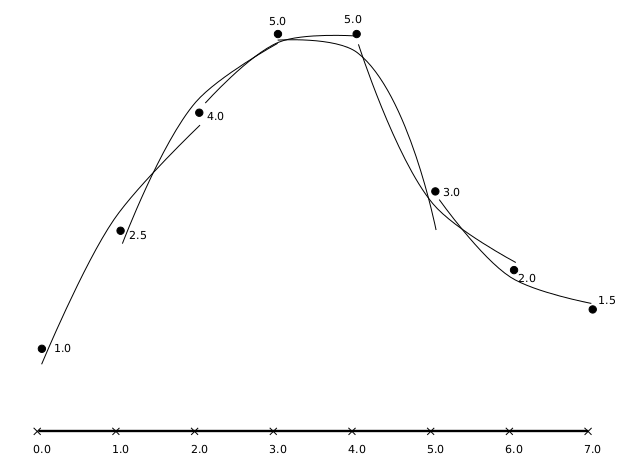
\includegraphics[width=0.7\textwidth]{figures/WLLS.png}
	\end{center}
	\caption{Weighted Local Least Squares fit for given data. Note the overlapping approximations at most points (\cite{MLSIntro})}
	\label{fig:WLLS}
\end{figure}
Unlike the Weighted Global Least Squares fit, there isn’t necessarily only one approximate solution at any point x in the domain since the neighborhoods of the local solutions overlap. Then the first choice we have for evaluating $u(x)$ is to use the local solution $u_p(x)$ at the point $x_p$. The other method could be averaging all solutions, which were calculated for point $x_p$ within its neighbors:
\begin{equation}
	u(x) = \dfrac{1}{n} \sum_{i=1}^n{u_i(x)}
\end{equation}
An example of what quadratic functions fitted to each point and its neighbors might look like is shown in Figure \ref{fig:WLLS}

More discussion on the MLS for an arbitrary point in space and Local Regression estimator could be found in \cite{MLSIntro}. In this thesis, the WLLS approach will be used to correct the SDF of the MC grid domain.

